% Prezentare CFAR-STFT Detecția Radarului
% Autori: Ingrid Corobana, Teodora Nae
% Compilare: pdflatex presentation_ro.tex (de 2 ori pentru TOC)

\documentclass[12pt,aspectratio=169]{beamer}

\usepackage[utf8]{inputenc}
\usepackage[romanian]{babel}
\usepackage{amsmath}
\usepackage{amssymb}
\usepackage{graphicx}
\usepackage{tikz}
\usepackage{xcolor}
\usepackage{hyperref}
\usepackage{booktabs}
\usepackage{multicol}

% Tema și culori
\usetheme{Madrid}
\usecolortheme{default}

\definecolor{stftblue}{RGB}{66, 133, 244}
\definecolor{cfarorange}{RGB}{255, 152, 0}
\definecolor{dbscangreen}{RGB}{76, 175, 80}
\definecolor{darkblue}{RGB}{25, 50, 100}
\definecolor{ipixpurple}{RGB}{156, 39, 176}

\setbeamercolor{structure}{fg=darkblue}
\setbeamercolor{alerted text}{fg=cfarorange}
\setbeamercolor{example text}{fg=dbscangreen}

% Calea pentru imagini
\graphicspath{{../results/ipix_figures/}{../results/animations/}{images/}}

\title[CFAR-STFT]{Analiza semnalelor radar în prezența ecourilor marine}
\subtitle{Abordare CFAR-STFT cu adaptări pentru sea clutter real}
\author[Corobana, Nae]{Ingrid Corobana \and Teodora Nae}
\date{Procesarea Semnalelor -- 2026}
\institute[FMI]{Universitatea din București\\Facultatea de Matematică și Informatică\\[0.3em]
Coordonator: Conf. Dr. Cristian Rusu}

\begin{document}

% ============================================================================
% SLIDE 1: TITLU
% ============================================================================
\begin{frame}
\titlepage
\end{frame}

% ============================================================================
% SLIDE 2: CUPRINS
% ============================================================================
\begin{frame}{Cuprins}
\tableofcontents
\end{frame}

% ============================================================================
% SECȚIUNEA 1: INTRODUCERE
% ============================================================================
\section{Introducere și Motivație}

\begin{frame}{Problema: Detecția în Sea Clutter}
\begin{columns}[T]
\column{0.55\textwidth}
\textbf{Ce este sea clutter?}
\begin{itemize}
    \item Ecouri radar de la suprafața mării
    \item Valuri, spumă, picături de apă
    \item \alert{Nu este Gaussian!} $\rightarrow$ Pondere mai mare în cozi
    \item Concentrat în jurul 0 Hz (Doppler mic)
\end{itemize}

\vspace{0.5em}
\textbf{Provocări:}
\begin{itemize}
    \item Statistici non-Gaussiene (K-distribution)
    \item Corelație temporală (valuri structurate)
    \item Ținte mici ascunse în clutter
\end{itemize}

\column{0.45\textwidth}
\begin{figure}
\includegraphics[width=\textwidth]{ipix_seaclutter_explanation.png}
\caption{\tiny Spectrogramă IPIX cu sea clutter}
\end{figure}
\end{columns}
\end{frame}

\begin{frame}{Soluția: CFAR-STFT (Abratkiewicz 2022)}
\textbf{Ideea cheie}: Exploatăm structura \alert{timp-frecvență}!

\vspace{0.5em}
\begin{enumerate}
    \item \textbf{STFT} $\rightarrow$ Reprezentare 2D (spectrogramă)
    \item \textbf{CFAR 2D} $\rightarrow$ Detecție adaptivă local
    \item \textbf{DBSCAN} $\rightarrow$ Clustering puncte detectate
    \item \textbf{Dilatare geodezică} $\rightarrow$ Extindere mască
    \item \textbf{iSTFT} $\rightarrow$ Reconstrucție semnal
\end{enumerate}

\vspace{0.5em}
\textbf{Contribuțiile noastre}:
\begin{itemize}
    \item Implementare completă în Python
    \item \alert{Adaptări pentru sea clutter real}: K-distribution, Hurst boost, DBSCAN asimetric
    \item Validare pe date IPIX reale
\end{itemize}
\end{frame}

% ============================================================================
% SECȚIUNEA 2: FUNDAMENTE TEORETICE
% ============================================================================
\section{Fundamente Teoretice}

\begin{frame}{STFT -- Transformata Fourier cu Timp Scurt}
\begin{equation*}
X(k,n) = \sum_{m=0}^{N-1} x(m) \cdot w(m - nH) \cdot e^{-j2\pi km/N}
\end{equation*}

\begin{columns}[T]
\column{0.5\textwidth}
\textbf{Parametri:}
\begin{itemize}
    \item $N_{fft} = 256$ (pentru IPIX)
    \item Hop $H = 32$ (87.5\% overlap)
    \item Fereastră Gaussiană $\sigma = 8$
\end{itemize}

\column{0.5\textwidth}
\textbf{De ce STFT?}
\begin{itemize}
    \item Localizare timp-frecvență
    \item Semnalele radar = ridges în TF
    \item Clutter-ul = energie difuză
\end{itemize}
\end{columns}

\vspace{0.5em}
\begin{block}{Two-sided pentru date complexe I/Q}
Date IPIX = I + jQ $\Rightarrow$ Frecvențe Doppler pozitive (apropiere) și negative (depărtare)
\end{block}
\end{frame}

\begin{frame}{GOCA-CFAR 2D -- Detecție Adaptivă}
\begin{columns}[T]
\column{0.5\textwidth}
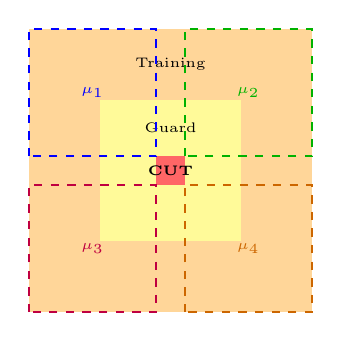
\begin{tikzpicture}[scale=0.45]
    % Training cells
    \fill[cfarorange!40] (-4,-4) rectangle (4,4);
    % Guard cells
    \fill[yellow!40] (-2,-2) rectangle (2,2);
    % CUT
    \fill[red!60] (-0.4,-0.4) rectangle (0.4,0.4);
    
    \node at (0,0) {\tiny\textbf{CUT}};
    \node at (0,1.2) {\tiny Guard};
    \node at (0,3) {\tiny Training};
    
    % GOCA quadrants
    \draw[blue, dashed, thick] (-4,0.4) rectangle (-0.4,4);
    \draw[green!70!black, dashed, thick] (0.4,0.4) rectangle (4,4);
    \draw[purple, dashed, thick] (-4,-4) rectangle (-0.4,-0.4);
    \draw[orange!80!black, dashed, thick] (0.4,-4) rectangle (4,-0.4);
    
    \node[blue, font=\tiny] at (-2.2,2.2) {$\mu_1$};
    \node[green!70!black, font=\tiny] at (2.2,2.2) {$\mu_2$};
    \node[purple, font=\tiny] at (-2.2,-2.2) {$\mu_3$};
    \node[orange!80!black, font=\tiny] at (2.2,-2.2) {$\mu_4$};
\end{tikzpicture}

\column{0.5\textwidth}
\textbf{GOCA = Greatest-Of Cell Averaging}
\begin{align*}
\hat{Z} &= \max(\mu_1, \mu_2, \mu_3, \mu_4) \\
T &= R \cdot \hat{Z} \\
R &= N_T (P_f^{-1/N_T} - 1)
\end{align*}

\textbf{Decizie}:
$$|X(k,n)|^2 \geq T \Rightarrow \text{\color{dbscangreen}Detectat}$$
\end{columns}

\vspace{0.3em}
\begin{alertblock}{Parametri IPIX}
$N_G = 3$, $N_T = 12$, $P_f = 0.001$ (mult mai mic decât paper!)
\end{alertblock}
\end{frame}

\begin{frame}{De ce CFAR nu detectează „toată zona albă"?}
\textbf{Observație}: De ce doar puncte localizate și nu regiuni uniforme?

\vspace{0.5em}
\begin{columns}[T]
\column{0.5\textwidth}
\textbf{Prag global (naiv)}:
\begin{itemize}
    \item Detectează tot peste -20 dB
    \item $\Rightarrow$ Mii de alarme false!
\end{itemize}

\column{0.5\textwidth}
\textbf{CFAR local-adaptiv}:
\begin{itemize}
    \item Compară cu \alert{vecinii locali}
    \item Zonă uniformă $\Rightarrow$ nu detectează
    \item Doar \alert{tranziții bruște} de putere
\end{itemize}
\end{columns}

\vspace{0.5em}
\begin{block}{Consecință}
CFAR detectează: margini, ridges, ținte reale -- NU zone omogene de clutter!
\end{block}
\end{frame}

% ============================================================================
% SECȚIUNEA 3: ADAPTĂRI SEA CLUTTER
% ============================================================================
\section{Adaptări pentru Sea Clutter}

\begin{frame}{Adaptarea 1: K-Distribution}
\textbf{Problema}: Sea clutter NU e Gaussian -- are \alert{spike-uri frecvente}!

\begin{equation*}
p(x) = \frac{4}{\Gamma(\nu)} \left(\frac{\nu x^2}{2\mu}\right)^{(\nu+1)/2} K_{\nu-1}\left(\sqrt{\frac{2\nu x^2}{\mu}}\right)
\end{equation*}

\begin{columns}[T]
\column{0.5\textwidth}
\textbf{Parametri}:
\begin{itemize}
    \item $\nu$ = parametru de formă
    \item $\nu$ mic $\Rightarrow$ mai „spiky"
    \item Estimare: $\nu = \mu^2/(\sigma^2 - \mu^2)$
\end{itemize}

\column{0.5\textwidth}
\textbf{Soluție}:
\begin{itemize}
    \item Estimăm $\nu$ din training cells
    \item Ajustăm multiplicatorul pragului
    \item Reducem alarme false în clutter
\end{itemize}
\end{columns}
\end{frame}

\begin{frame}{Adaptarea 2: Fractal Boost (Hurst)}
\textbf{Problema}: CFAR poate rata ținte slabe sub prag

\vspace{0.3em}
\textbf{Observație}: Sea clutter are proprietate \alert{fractală} (self-similar)

\begin{equation*}
\mathbb{E}\left[|X(t+\tau) - X(t)|^2\right] \propto \tau^{2H}
\end{equation*}

\begin{itemize}
    \item Sea clutter: $H \approx 0.75$--$0.85$ (persistent)
    \item Când apare țintă: structura se perturbă, $H$ scade sub $\sim 0.6$
\end{itemize}

\vspace{0.3em}
\begin{block}{Soluție}
Calculăm $H$ per bin de frecvență. Dacă $H < 0.6$ și putere mare $\Rightarrow$ potențială țintă!
$$\text{mască} = \text{CFAR} \lor (\text{anomalie Hurst} \land \text{putere mare})$$
\end{block}
\end{frame}

\begin{frame}{Adaptarea 3: DBSCAN Asimetric}
\textbf{Problema}: Țintele apar ca semnături aproape verticale în spectrogramă (energie pe multe binuri de frecvență, pe puține cadre temporale)

\vspace{0.5em}
DBSCAN standard tinde să fragmenteze aceste semnături în mai multe clustere atunci când există discontinuități.

\vspace{0.5em}
\textbf{Soluție}: Metrica de distanță asimetrică cu scalare pe frecvență ($s_f = 3.0$):
\begin{equation*}
d = \sqrt{(\Delta t)^2 + \left(\frac{\Delta f}{s_f}\right)^2} \quad \text{cu } s_f = 3.0
\end{equation*}

\vspace{0.3em}
\textbf{Impact}: Ținta întinsă pe aproximativ 50 binuri de frecvență $\Rightarrow$ \alert{un singur cluster coerent}

\vspace{0.5em}
\begin{columns}[T]
\column{0.5\textwidth}
\textbf{Alte adaptări}:
\begin{itemize}
    \item Mascare componentă DC: ±8 binuri (≈±31 Hz)
    \item Filtru bandwidth Doppler: BW ≥ 2 binuri (≈8 Hz)
\end{itemize}
\column{0.5\textwidth}
\end{columns}
\end{frame}

% ============================================================================
% SECȚIUNEA 4: REZULTATE
% ============================================================================
\section{Rezultate Experimentale}

\begin{frame}{Rezultate pe Date Sintetice (Chirp Neliniar)}
\begin{table}
\centering
\begin{tabular}{cccc}
\toprule
\textbf{SNR [dB]} & \textbf{RQF\_mean [dB]} & \textbf{RQF\_std} & \textbf{Detecție [\%]} \\
\midrule
5 & 7.28 & 0.47 & 100 \\
10 & 16.81 & 0.60 & 100 \\
15 & 22.95 & 0.56 & 100 \\
20 & 26.40 & 0.51 & 100 \\
25 & 28.43 & 0.39 & 100 \\
30 & \textbf{29.17} & 0.25 & 100 \\
\bottomrule
\end{tabular}
\end{table}

\begin{itemize}
    \item 100 rulări Monte Carlo per nivel SNR
    \item Rata de detecție: 100\% în toate cazurile experimentale
    \item RQF crește monoton cu SNR pentru semnalul sintetic studiat
\end{itemize}
\end{frame}

\begin{frame}{Detecție pe Date IPIX Reale}
\begin{columns}[T]
\column{0.55\textwidth}
\textbf{Baza de date IPIX (McMaster University, 1993)}:
\begin{itemize}
    \item Radar X-band: $f_{RF} = 9.39$ GHz
    \item PRF = 1000 Hz
    \item Semnale complexe I/Q
    \item Țintă de calibrare: sferă 1 m la distanța de 2660 m
\end{itemize}

\vspace{0.5em}
\textbf{Relație Doppler -- Viteză radială}:
$$v_r = \frac{f_d \cdot c}{2 f_{RF}}$$
Exemplu: $f_d = 100$ Hz $\Rightarrow$ $v_r \approx 1.6$ m/s

\column{0.45\textwidth}
\begin{figure}
\includegraphics[width=\textwidth]{ipix_target_17_goca_frame83.png}
\caption{\tiny Detecție GOCA-CFAR pe Target \#17}
\end{figure}
\end{columns}
\end{frame}

\begin{frame}{Detecție cu Fractal Boost}
\begin{figure}
\centering
\includegraphics[width=0.85\textwidth]{ipix_target_17_fractal_frame83.png}
\caption{GOCA-CFAR + Fractal Boost pe IPIX Target \#17 -- Îmbunătățește detecția țintelor slabe}
\end{figure}
\end{frame}

\begin{frame}{Animații de Detecție (GIF-uri)}
\textbf{Disponibile în repository}:

\vspace{0.5em}
\begin{itemize}
    \item \texttt{ipix\_target\_17\_goca\_*.gif} -- Detecție cu metoda GOCA standard
    \item \texttt{ipix\_target\_17\_fractal\_boost\_*.gif} -- Cu amplificare Hurst (anomalie fractală)
    \item \texttt{ipix\_target\_17\_asymmetric\_*.gif} -- Cu DBSCAN asimetric
    \item \texttt{ipix\_target\_30\_detection.gif} -- Target \#30 (sea state ridicat)
\end{itemize}

\vspace{0.5em}
\begin{block}{Vizualizare animații}
Animațiile arată evoluția detecțiilor în timp, cu suprapunerea măștilor CFAR și semnalelor detectate pe spectrograma STFT.
\end{block}

\vspace{0.3em}
\small\texttt{https://github.com/dirgnic/Radar\_Detection\_STFT/tree/main/results/animations}
\end{frame}

% ============================================================================
% SECȚIUNEA 5: COMPARAȚIE PARAMETRI
% ============================================================================
\section{Comparație Parametri}

\begin{frame}{Parametri: Paper vs. Implementare}
\begin{table}
\centering
\small
\begin{tabular}{lccc}
\toprule
\textbf{Parametru} & \textbf{Paper} & \textbf{Sintetic} & \textbf{IPIX (real)} \\
\midrule
$f_s$ & 12.5 MSa/s & 12.5 MSa/s & 1000 Hz (PRF) \\
$N_{fft}$ & 512 & 512 & 256 \\
Fereastră STFT & Gauss $\sigma=8$ & Gauss $\sigma=8$ & Gauss $\sigma=8$ \\
Hop & -- & 256 & 32 \\
$N_G$ & 16 & 16 & \alert{3} \\
$N_T$ & 16 & 16 & \alert{12} \\
$P_f$ & 0.4 & 0.4 & \alert{0.001} \\
Model clutter & Gaussian & Gaussian & \alert{K-distribution} \\
DBSCAN $\varepsilon$ & -- & 8 & 8 \\
freq\_scale & -- & 1.0 & \alert{3.0} \\
\bottomrule
\end{tabular}
\end{table}

\textbf{Modificări cheie pentru sea clutter}: $P_f$ mult mai mic, K-distribution, DBSCAN asimetric
\end{frame}

% ============================================================================
% SECȚIUNEA 6: CONCLUZII
% ============================================================================
\section{Concluzii}

\begin{frame}{Concluzii și Contribuții}
\begin{enumerate}
    \item \textbf{Implementare completă} CFAR-STFT în Python cu API flexibil
    \item \textbf{Validare pe date sintetice}: RQF = 29.17 dB la SNR=30 dB; rata detecție 100\% în 100 rulări Monte Carlo
    \item \textbf{Validare pe date reale}: Detecții consistente pe secvențe IPIX (Target \#17, \#30, \#40)
    \item \textbf{Adaptări pentru sea clutter real}:
    \begin{itemize}
        \item K-distribution pentru modelarea statisticilor non-Gaussiene
        \item Amplificare prin anomalie Hurst pentru sensibilitate crescută la ținte slabe
        \item DBSCAN asimetric pentru coerența semnăturilor verticale în timp-frecvență
    \end{itemize}
    \item \textbf{Performanță}: aproximativ 75 ms/segment pe CPU (13 FPS pentru fereastră 2s, hop 0.5s)
\end{enumerate}

\vspace{0.5em}
\begin{block}{Reproducibilitate}
Cod și date: \url{https://github.com/dirgnic/Radar_Detection_STFT}
\end{block}
\end{frame}

\begin{frame}{Direcții Viitoare}
\begin{itemize}
    \item \textbf{Accelerare GPU}: CUDA/OpenCL pentru timp real
    \item \textbf{Optimizare automată}: ML pentru calibrare parametri
    \item \textbf{Multi-target tracking}: Predicție traiectorii
    \item \textbf{Integrare sistem real}: Radar operațional
\end{itemize}

\vspace{1.5em}
\begin{center}
{\Large \textbf{Mulțumim pentru atenție!}}

\vspace{0.5em}
{\large Întrebări?}
\end{center}
\end{frame}

% ============================================================================
% BACKUP SLIDES
% ============================================================================
\appendix

\begin{frame}{Backup: Formula RQF}
\textbf{Reconstruction Quality Factor}:
\begin{equation*}
\text{RQF} = 10 \log_{10}\left(\frac{\sum_n |x[n]|^2}{\sum_n |x[n] - \hat{x}[n]|^2}\right) \text{ [dB]}
\end{equation*}

\begin{itemize}
    \item $x[n]$ = semnal original (curat)
    \item $\hat{x}[n]$ = semnal reconstruit
    \item RQF mai mare $\Rightarrow$ reconstrucție mai bună
\end{itemize}
\end{frame}

\begin{frame}{Backup: Interpretare Doppler IPIX}
\begin{columns}[T]
\column{0.5\textwidth}
\textbf{Two-sided spectrum}:
\begin{itemize}
    \item $f_d > 0$ $\Rightarrow$ țintă se apropie
    \item $f_d < 0$ $\Rightarrow$ țintă se depărtează
    \item $f_d \approx 0$ $\Rightarrow$ sea clutter
\end{itemize}

\column{0.5\textwidth}
\textbf{Pentru IPIX}:
\begin{align*}
v_{max} &= \frac{PRF \cdot c}{4 f_{RF}} \\
&\approx \pm 8 \text{ m/s}
\end{align*}
\end{columns}
\end{frame}

\end{document}
